\chapter{Implementation}
@todo How the source was designed and maintained. Mention that the development of the code can be found on Github?


\section{ECMAScript}
ECMAScript \footnote{http://www.ecmascript.org/} is a standardized scripting language widely used in website development. Latest approved edition of ECMAScript is ECMAScript 5.1, which is implemented in most major web browsers, and is commonly called JavaScript \footnote{https://developer.mozilla.org/en/docs/Web/JavaScript} \footnote{https://msdn.microsoft.com/cs-cz/library/d1et7k7c(v=vs.94).aspx}. 

JavaScript is a dynamic programming language \footnote{http://en.wikipedia.org/wiki/Dynamic\_programming\_language}, which combines multiple aspects of imperative, functional, and object-oriented programming.

Functions are so called first-class citizens. This means they can be stored in variables, passed as function parameters, returned as results of functions, and included in data structures \cite{}\footnote{http://mitpress.mit.edu/sicp/full-text/book/book-Z-H-12.html\#call\_footnote\_Temp\_121}.

Object oriented programming (OOP) \footnote{http://en.wikipedia.org/wiki/Object-oriented\_programming} in JavaScript differs from class-oriented OOP in the way inheritance is implemented. While in class-oriented languages, for example in C++ or C\#, inheritance is achieved by declaring classes of objects. In JavaScript, object prototypes are used to implement this functionality. @todo

JavaScript doesn't provide any mean of static type checking. All types are created during runtime and they are also checked only during runtime. This lack of static checking during compilation might lead to rarely occurring errors and it is important to take this in mind while writing JavaScript code. A good practice is to write documentation comments\footnote{Commonly used syntax in JavaScript projects is JSDoc (http://usejsdoc.org/)}, where the types are stated.

JavaScript is an interpreted language, some implementations also use a Just-in-time compilation (JIT) \footnote{For example Google V8 engine used in Google Chrome. See https://code.google.com/p/v8/} for better performance. 

Another very important aspect of ECMAScript which affects it's performace is the absence of direct control over memory usage -- a garbage collector frees unused .

\subsection{TypeScript}
TypeScript is a typed superset of JavaScript that compiles to plain JavaScript\cite{} \footnote{http://www.typescriptlang.org/}. It is an open-source project developed by Microsoft. It is, as it's name suggests, is a strongly typed programming language compatible with JavaScript.

TypeScript extends capabilities of JavaScript by static type checking in the time of compilation, which helps finding errors in source code, and speeds up the process of coding. TypeScript also introduces class-based object oriented programming to JavaScript. It includes concepts of interfaces and polymorphism, which makes programs written in TypeScript more understandable to programmers familiar with other object-oriented programming languages like Java, C\# or C++.

TypeScript is transcompiled into regular JavaScript, and therefore doesn't bring any new functionality. The reason for choosing TypeScript is the clarity of code and more convenient development process for the programmer.

\section{Event driven programming}
The idea behind event driven programming is to break direct references between objects and to communicate with \textit{events} instead of calling object methods directly. The advantage of the this approach is loose coupling \footnote{http://en.wikipedia.org/wiki/Coupling\_(computer\_programming)} -- features might be added or removed without breaking the core of the application.

Each object handles only it's own task without knowing anything about the other objects it's collaborating with. When an object completes it's task, it publishes the result with a specific event. Objects subscribed for this event are notified and are given the outcomes of the previous task.

This mechanism is sometimes called the \textit{Event Aggregator} design pattern \cite{}. It is implemented through the \textit{VideoEvents}\footnote{Implementation can be found in \textit{/public/js/app/Helpers/VideoEvents.ts} file} static class, which makes it a simple singleton object. This class provides an interface for registering and triggering callbacks for specified events. Callbacks executed by a triggered event are called asynchronously. It is worth mentioning that web browsers execute all scripts in a single thread.

\begin{verbatim}
VideoEvents.on(VideoEventType.Message, function(message) {
	console.log("received message:", message);
});

VideoEvents.on(VideoEventType.Message, function(message) {
	console.log("received message backwards:", message.split("").reverse().join(""));
});

VideoEvents.trigger(VideoEventType.Message, "Hello world.");
\end{verbatim}

Events triggered and expected by each object are described in the programmer's documentation and can be used to extend the behavior of the player or the recording tool without modifying the original source code.




\section{HTML5}

What is HTML5, what parts are needed. Compatibility of these technologies in browsers. A chart of people using a compatible browser? Playing should be possible in the vast majority of browsers today and the prognosis is good.

\subsection*{Web workers}
Multi-threading in JavaScript. Async methods and web workers.

\subsection*{Working with XML data}
The XMLDocument object.



\subsection{Rendering graphics using HTML5}

Displaying text and static visual content is the main purpose of HTML and Cascade Style Sheets (CSS) and it is widely used this way across the web. Creating a complex polygon or curve would be very hard and would involve various tricks \footnote{http://nicolasgallagher.com/pure-css-gui-icons/} or would be even impossible. 

The new HTML specification takes this in mind and brings ways of creating more rich and dynamic content within a web page. There are two technologies that should be taken into account - Canvas 2D Context and SVG.

\paragraph{Canvas 2D Context}
The Canvas element provides scripts with a resolution-dependent bitmap canvas, which can be used for rendering graphs, game graphics, or other visual images on the fly \cite{} \footnote{http://www.w3.org/TR/2010/WD-html5-20100624/the-canvas-element.html}. 

Using canvas seems appropriate for this project. Canvas could be created with respect to user's resolution and web browser window size. All elements can be scaled to fit this viewport. This will make them look sharp and there won't be any artifacts, noise and blur caused by interpolation which would be caused by scaling normal bitmap video.

The problem with Canvas might occur when user resizes his window or enters full-screen after the canvas is initialized. Canvas contains a bitmap image consisting of graphical primitives drawn onto it. All content must be redrawn so it remains sharp.

\paragraph{Scalable Vector Graphics (SVG)}
Scalable Vector Graphics (SVG)\footnote{http://www.w3.org/TR/SVG/} is an XML (Extensible Markup Language) based file format designed for describing two-dimensional vector images. It is an open format developed and maintained by the W3C SVG Working Group \cite{} . Current W3C recommendation is SVG 1.1 (Second Edition).

A valid SVG document must have an \textit{svg} root element with specific namespace attributes and specified \textit{width} and \textit{height} attributes. An example of an empty, but valid, SVG document might look as shown:

\begin{verbatim}
<?xml version="1.0"?>
<svg version="1.1"
        width="470"
        height="100"
        xmlns="http://www.w3.org/2000/svg"
        xmlns:xlink="http://www.w3.org/1999/xlink"
        xmlns:ev="http://www.w3.org/2001/xml-events">

</svg>

\end{verbatim}

The specification of SVG introduces several graphical primitives, that can be used to compose complex shapes. Each primitive is represented by an XML element and a set of attributes. The list of primitives is long, though we will need only two of them -- the \textit{circle} and \textit{path}.

A circle needs three basic properties -- \textit{cx} and \textit{cy} (coordinates of it's center) and it's radius \textit{r}. Other attributes, like \textit{fill} or \textit{stroke}, can be used to specify the appearance of the primitive. For example a black dot with it's center at point \textit{\[50, 50\]} and radius of 50 would be represented by this XML element:

\begin{verbatim}
<circle cx="50" cy="50" r="50" fill="black" />
\end{verbatim}



\subsection{Audio capturing, processing and upload}

HTML5 provides only one way to access microphone data at the moment and it is through the \textit{getUserMedia API} \footnote{getUserMedia: http://www.w3.org/TR/mediacapture-streams/\#dom-mediadevices-getusermedia} \cite{}. \textit{navigator.getUserMedia} function prompts the user to for permission to use their audio input (this function is also used to access webcam stream in other applications). The \textit{navigator.getUserMedia} function is well documented on Mozilla Developer Network (MDN) \footnote{MDN: https://developer.mozilla.org/en-US/docs/Web/API/Navigator/getUserMedia} website.

If user's device has a connected microphone and user gives his permission to use his audio input, then a \textit{MediaStream} \footnote{MediaStream: http://www.w3.org/TR/mediacapture-streams/\#idl-def-MediaStream} object is provided by the browser and from this time on audio can be captured. Error callback with \textit{MediaStreamError}\footnote{MediaStreamError: http://www.w3.org/TR/mediacapture-streams/\#idl-def-MediaStreamError} instance is called otherwise.

Once the \textit{MediaStream} is obtained, 

\subsection{AJAX}

%\subsection{}


\subsection{High Resolution Timer}
To make the video look as good as possible, we need to store as precise data as possible. The \textit{Date.now()} function\footnote{https://developer.mozilla.org/en-US/docs/Web/JavaScript/Reference/Global\_Objects/Date/now} returns the number of milliseconds elapsed since 1 January 1970 00:00:00 UTC. The millisecond accuracy might seem enough, but modern browsers provide even more accurate data via the \textit{High Resolution Time} \footnote{https://dvcs.w3.org/hg/webperf/raw-file/tip/specs/HighResolutionTime/Overview.html} via the \textit{window.performance.now()} function\footnote{https://developer.mozilla.org/en-US/docs/Web/API/Performance/now} \footnote{http://updates.html5rocks.com/2012/08/When-milliseconds-are-not-enough-performance-now} with the accuracy of microseconds. The \textit{window.performance.now()} function doesn't provide data related to current time, but the milliseconds elapsed since page was loaded as a floating point number. This makes it more suitable for animation purposes.

Timing functionality is wrapped in \textit{VideoTimer} class\footnote{implementation can be found in \textit{/public/js/app/Helpers/VideoTimer.ts} file} with a method for getting the number of milliseconds elapsed since last timer reset with the best precision provided by the web browser.

\subsection{Input from pointing devices}

Detecting mouse movement and the state of it's buttons is a very common task in web development. Users navigate through web pages mainly by clicking on hypertext links with their computer mouse. Therefore mouse events are well specified and work across all desktop web browsers and desktop platforms.

Unfortunately, the situation among other pointing devices other than computer mice is much less uniform. With the boom of smartphones and tablets, touchscreens are very common. Also computer graphics tablets are used by artists and many people use them when creating a Khan Academy style video.

\subsubsection{Wacom Webplugin pen API}
The Wacom Webplugin pen API (WebPAPI) is a browser plugin interface for pen data access from all Wacom consumer and professional tablets \cite{}\footnote{http://www.wacomeng.com/web/WebPluginReleaseNotes.htm}.

Unfortunatelly support for this plugin was discontinued by Chromium and Google Chrome \footnote{http://blog.chromium.org/2013/09/saying-goodbye-to-our-old-friend-npapi.htm} and therefore it should not be relied on.

\subsubsection{Touch Events API}
Touch Events API is an API for handling touch input from touch screens. The standard is proposed by Apple and is implemented across many platforms and in many mobile web browsers \footnote{http://caniuse.com/\#feat=touch} \cite{}.

This API supports multiple touches at once, but this feature is not needed and neither implemented in this project. Unfortunately, this API provides no touch pressure information.

\subsubsection{Pointer Events API}
Pointer Events API is an open API created by Microsoft. It's purpose is to unify the way mouse events, touch screen events, stylus and other (i.e. Kinect) similar ways into one API. This technology is implemented in Internet Explorer and will be also present in the final version of the Microsoft Edge browser. Firefox implements this API, but it is so far accessible only if a specific hidden flag is enabled. Google has announced the intent to also implement this functionality in upcoming releases of Google Chrome across all platforms.

This API also provides pressure information for pointing devices, that support this feature, including Wacom graphics tablets.


\section{Drawing curves}
Khan Academy videos are known for it's consistent and simple style. A person draws on a virtual canvas (evoking a school blackboard) with a brush (or possibly a chalk) of a round shape.

Tutor has a pointing device, typically a computer mouse or digital pen, and it's position on the canvas is marked with a moving cursor. When the tutor clicks, a dot is marked on canvas in the current position of the cursor. Tutor can produce a line (typically a curve) following this cursor when he presses a mouse button or increases digital pen pressure and while moving the cursor. The curve ends when he releases the button or pen pressure. The color and size of the dot or line corresponds to the current settings.

At the time of recording, mouse coordinates relative to the drawing board are captured along with current pressure of the digital pointing device (mouse, graphical tablet pen). This data is then used to draw a curve with variable thickness at the moment of recording as visual feedback for the person recording and the same process is done every time the video is replayed.

The outcome of the rendering phase should be the same every time so the intention of the creator is preserved. On the other hand, the rendering algorithm might be improved (i.e. by making the lines smoother) in the future and the video could be rendered using to this algorithm without any editing, while the information in the video will remain untouched.

Rendering at the time of playback gives us the opportunity to adjust the outcome to the environment of the end user. This means that the result can be sharp on every display resolution without the need of having many versions of the same video for each resolution.

\subsection{DynaDraw algorithm}

Paul Haeberli has created a simple algorithm called \textit{"DynaDraw"} in 1989, which is suitable for calligraphy. Brush is modeled as a physical object with it's mass, velocity and friction coefficient \footnote{DynaDraw: http://www.graficaobscura.com/dyna/index.html} \cite{}. Mouse movement is interpreted as a way of exerting force on the brush -- the faster you move the brush, the greater the force applied on the brush is. Acceleration is then calculated according to Newton's second law of motion considering brush's mass and velocity of the brush is derived with respect to the amount of brush's friction. This velocity is then applied and brush is moved. The trace brush should leave behind is then drawn onto the blackboard.

The advantage of this algorithm is it's simplicity and the possibilities of configuring the brush with different values of mass and friction (the author of the algorithm refers to this constant also as a drag, which better fits the purpose of slowing down the brush).

Heavier brushes move slowly, but the path they leave behind is much smoother, as the hand shaking is eliminated by composition of forces in different directions.

Light brushes move faster and are often very close to the cursor during the movement. When the cursor stops abruptly, light brushes with little friction tend to keep moving past the cursor and wrap around it. This produces little curls at the end of lines.

This approximation of cursor movement with appropriate constants selected improves quality of user's input and leads to nice results event when the user is using an ordinary mouse instead of a digital drawing pen.

\subsubsection*{Brush movement simulation}

One step of simulation applies force on the brush according to current mouse position and thus moves it in the direction of the pointer. This process of applying force must be  done periodically, at the frequency of 60 Hz in ideal case\footnote{HTML5 provides \textit\textit{requestAnimationFrame} function, which is intended for animations and which targets 60 frames per second}. Implementation of this simulation is not identical to the original \textit{DynaDraw} algorithm, but all of it's key aspects are preserved. Pseudocode ~\ref{alg:one-step} describes the algorithm used in this theses.

The main difference between the original implementation and the one used in Vector Video is brush width calculation. The original algorithm calculates the width of the line in a specific point by measuring it's velocity -- the faster the brush is moving, the thinner the drawn line is. This width dynamics gave the algorithm it's name.

In our implementation, this effect is implemented, but is much more subtle. Brush dynamic in this implementation relies mainly on the pressure of a digital pen on a graphics tablet. Since the exact value of pressure in the point of current brush's location is not always known, the value is linearly interpolated between the value of pressure in the previous position of the brush and the value of pressure in the current mouse position according to distance from each of these points.

As this simulation isn't deterministic, this process cannot be reconstructed afterwards and when the video is being played, only the already computed values of points along the path must be used. The precise value of pressure is therefore redundant for later playback of the video and 

\begin{pseudocode}
  \begin{algorithmic}

  \Function{OneStep}{$M$, $\Delta t$} \Comment $M$ - mouse position, $\Delta t$ - elapsed time
      \If {$M \neq \emptyset$}
	      \State $brushMoved \gets \Call{apply}{\vec{M}, \Delta t} $
          \If {$brushMoved = true$}
              \State \Call{DrawSegment}{}
          \EndIf
      \EndIf
 \EndFunction

\Function{apply}{$M, \Delta t$}
      \State $ \vec{F} \gets M - P $\Comment $P$ - current position of the brush
      \State $ \vec{a} = \frac{\vec{F}}{m} $\Comment $m$ - mass of the brush

      \If{$ \norm{\vec{a}} \le C_a $} \Comment $C_a$ - minimum acceleration constant
	      \State \Return false;    
       \EndIf
      
      \State $\vec{v} \gets \vec{v} + \vec{a}$

      \If {$ \norm{\vec{v}} > C_v$} \Comment $C_v$ - minimum velocity constant
          \State $ P \gets P + \mu\Delta t\vec{v} $\Comment $\mu$ - coefficient of friction
		  \State \Return true
      \EndIf
      \State \Return false
  \EndFunction
\end{algorithmic}
\caption{One step of brush movement simulation}
\label{alg:one-step}
\end{pseudocode}

\subsubsection*{Rendering of one line segment}

Line consists of many segments that are drawn after every simulation step, which causes brush to move. There are several ways to draw the segment, the most straightforward is to draw a simple quadrilateral between two points . as shown in Figure ~\ref{fig:draw-segment-quadrilateral} and Pseudocode ~\ref{alg:draw-segment-quadrilateral}.

	\begin{pseudocode}[H]
    	\begin{algorithmic}
        	\Function{DrawSegment}{}
                  \State $ \vec{n} \gets \frac{(-\vec{v}_y, \vec{v}_x)}{\norm{\vec{v}}} $        
                  \State $ w \gets \Call{CurrentBrushPressure}{} \cdot b $ \Comment $b$ - brush size
                  \State $L \gets P - w\vec{n}$
                  \State $R \gets P + w\vec{n}$

                  \State \Call{BeginPath}{}
                  \State \Call{MoveTo}{$L'$} \Comment $L'$ and $R'$ - previousely drawn point
                  \State \Call{LineTo}{$R'$}
                  \State \Call{LineTo}{$R$}
                  \State \Call{LineTo}{$L$}
                  \State \Call{ClosePath}{}
                  \State \Call{Fill}{c} \Comment c - current brush color

                  \State $L' \gets L$
                  \State $R' \gets R$
              \EndFunction
           \end{algorithmic}
      	   \caption{Draw one segment of a line}
          \label{alg:draw-segment-quadrilateral}
       \end{pseudocode}
       
      \begin{figure}
      	\centering
          %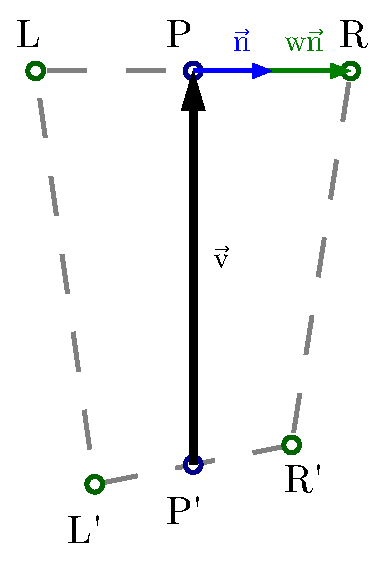
\includegraphics[width=30mm]{../img/draw-segment-quadrilateral.eps}
          \caption{Drawn segment - quadrilateral}
          \label{fig:draw-segment-quadrilateral}
      \end{figure}

@todo: splines, bezier curves, curved segment